\chapter{Head-on collisions of Xe and Cs}\label{ch:head-on-xece}
	\section{Introduction}\label{sec:intro-collisions}
		It is well established that helium droplets can readily capture in their interior almost any atom or molecule interacting with them, as first shown for the case of Ne atoms\citep{Sch90}, with the notable exception of alkali\citep{Sti96} and some alkaline-earth\citep{Her07} atoms. This property, together with the very low temperature $(T)$ achieved in helium droplets --- of the order of 0.4 K --- makes them the perfect ultracold and inert environment for hosting and studying isolated atoms and molecules, which is at the basis of current applications of helium droplets for spectroscopic studies of atoms and molecules. Besides, the superfluid nature of helium facilitates binary encounters of atoms/molecules in the bulk of the droplet while absorbing the energy released upon recombination, making possible chemical reactions which would not otherwise occur in the gas phase. These unique properties  of helium droplets have had a huge impact on their study\citep{Toe04,Sti06,Tig07,Cal11a,Mud14}.

		The pickup of Ar, Kr and Xe atoms in the gas phase by $^4$He$_N$ droplets with $N> 10^3$ atoms produced by nozzle beam expansions was studied about twenty years ago by Toennies and coworkers\citep{Lew95}. In these experiments the droplets in the helium beam were deflected by impacting with a secondary beam made of rare gas atoms in order to detect the pick-up. 

		Very recently, time-dependent density functional theory (TDDFT) has been used to address the capture of Cs or Ne atoms by $^4$He nanodroplets\citep{Lea14a,Vil16b}. The Cs capture was treated fully three dimensionally with the Cs atom described as a classical particle, whereas for the Ne capture study the Ne atom was described quantum-mechanically but the description was strictly one-dimensional.
			
		Motivated by recent experiments that use Xe atoms to visualise vortex arrays in very large helium droplets\citep{Gom14,Jon16}, we present here a first step towards the description of the capture  of Xe atoms by helium droplets, namely head-on collisions of Xe atoms against a $^4$He$_{1000}$ droplet. A discussion on the dynamic capture of Xe atoms by droplets hosting vortex lines and vortex arrays will be provided by a forthcoming study combining DFT simulation of vortex arrays as in\rfs{Anc14,Anc15} for helium nanocylinders and nanodroplets  and collision with Xe atoms as in this work. Whenever possible, the results for Xe, a heliophilic atom,  are contrasted with results for Cs, a heliophobic atom with similar mass. We use TD-DFT as described in \scn{sec:td-dft}. 

		\begin{figure}[!] 
			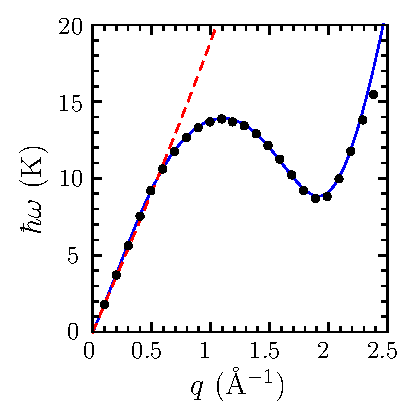
\includegraphics[width=1.0\linewidth,clip=true]{fig1}
			\caption{ \label{fig1-headon} Energy of the Xe@$^4$He$_{1000}$ complex as a function of the distance between  the Xe atom and the  COM of the droplet. Several two-dimensional helium densities and density profiles are shown for distances between 0 and 40 \AA{} in 5  \AA{} steps. Connected (dots) and disconnected (triangles) helium configurations are shown \emph{(see text)}. Top left inset: Snapshot of the helium density at the first turning point  during the dynamic evolution of a Xe atom (green dot) at $v_0 = 600$ m/s attained  78 ps after it has started. (Color figure online.)}
		\end{figure}

	\section{Results}

		\begin{figure}[!]
			\centerline{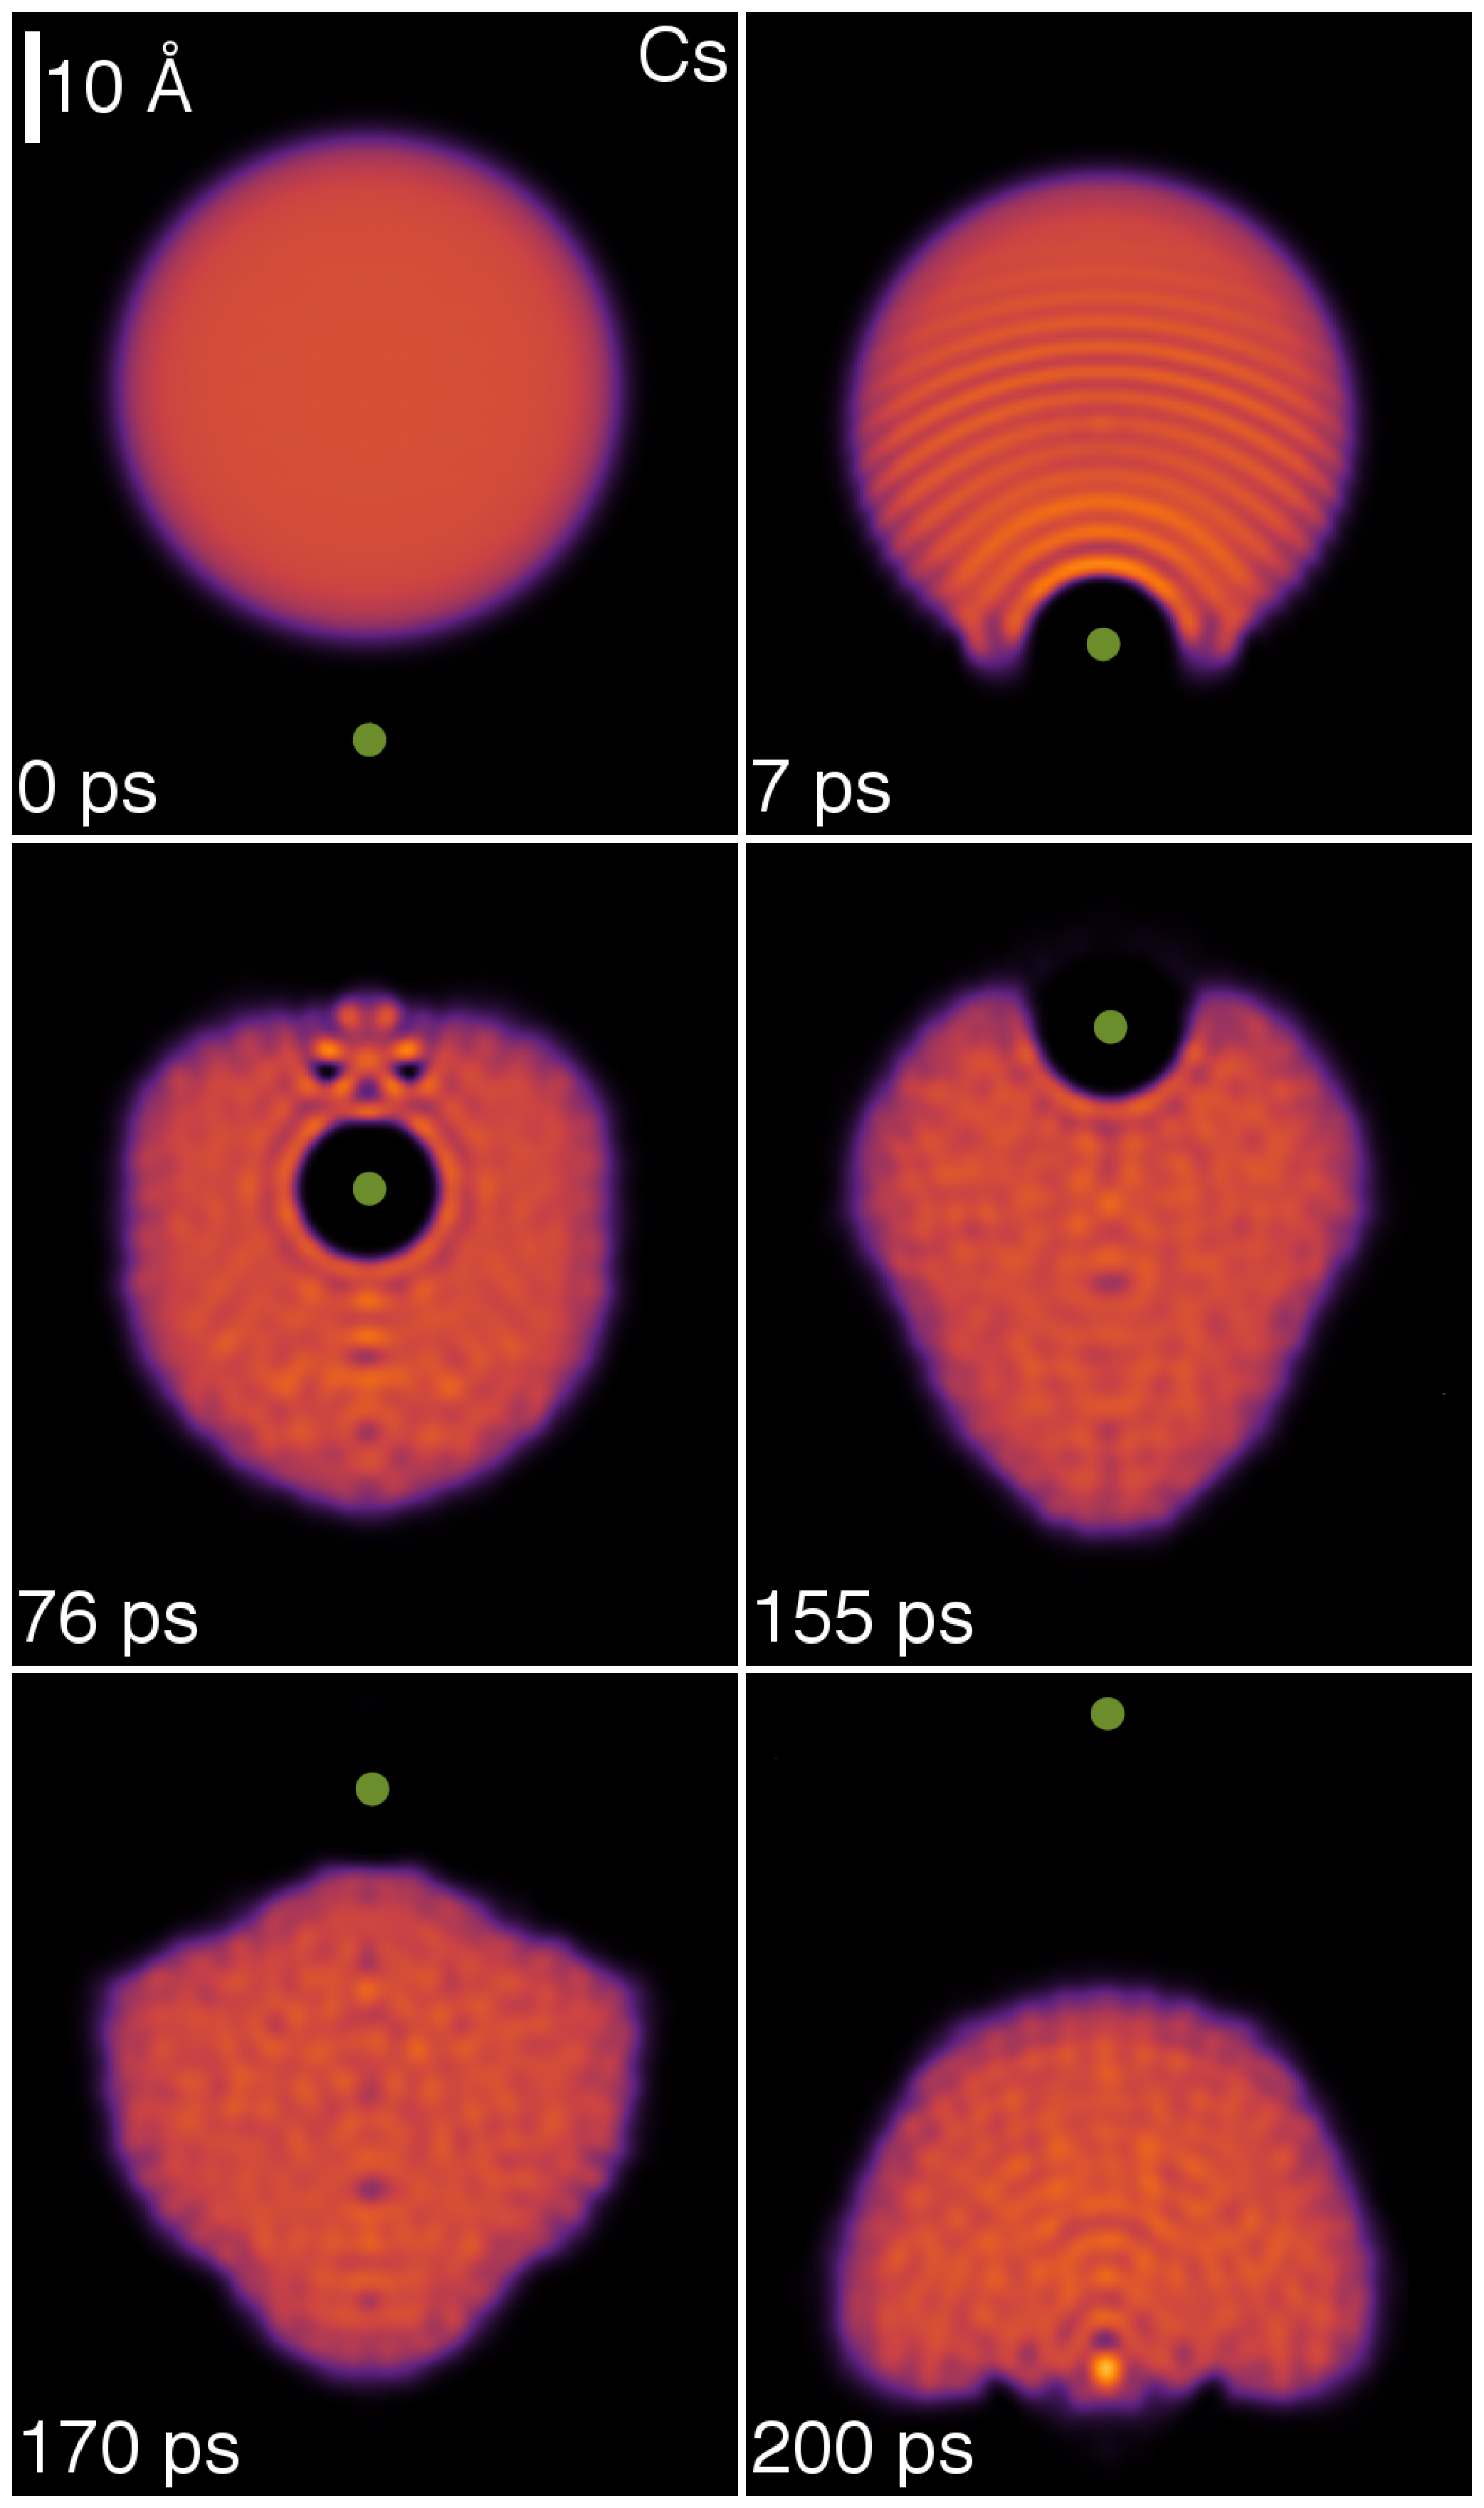
\includegraphics[width=0.50\linewidth,clip]{fig2-Cs} 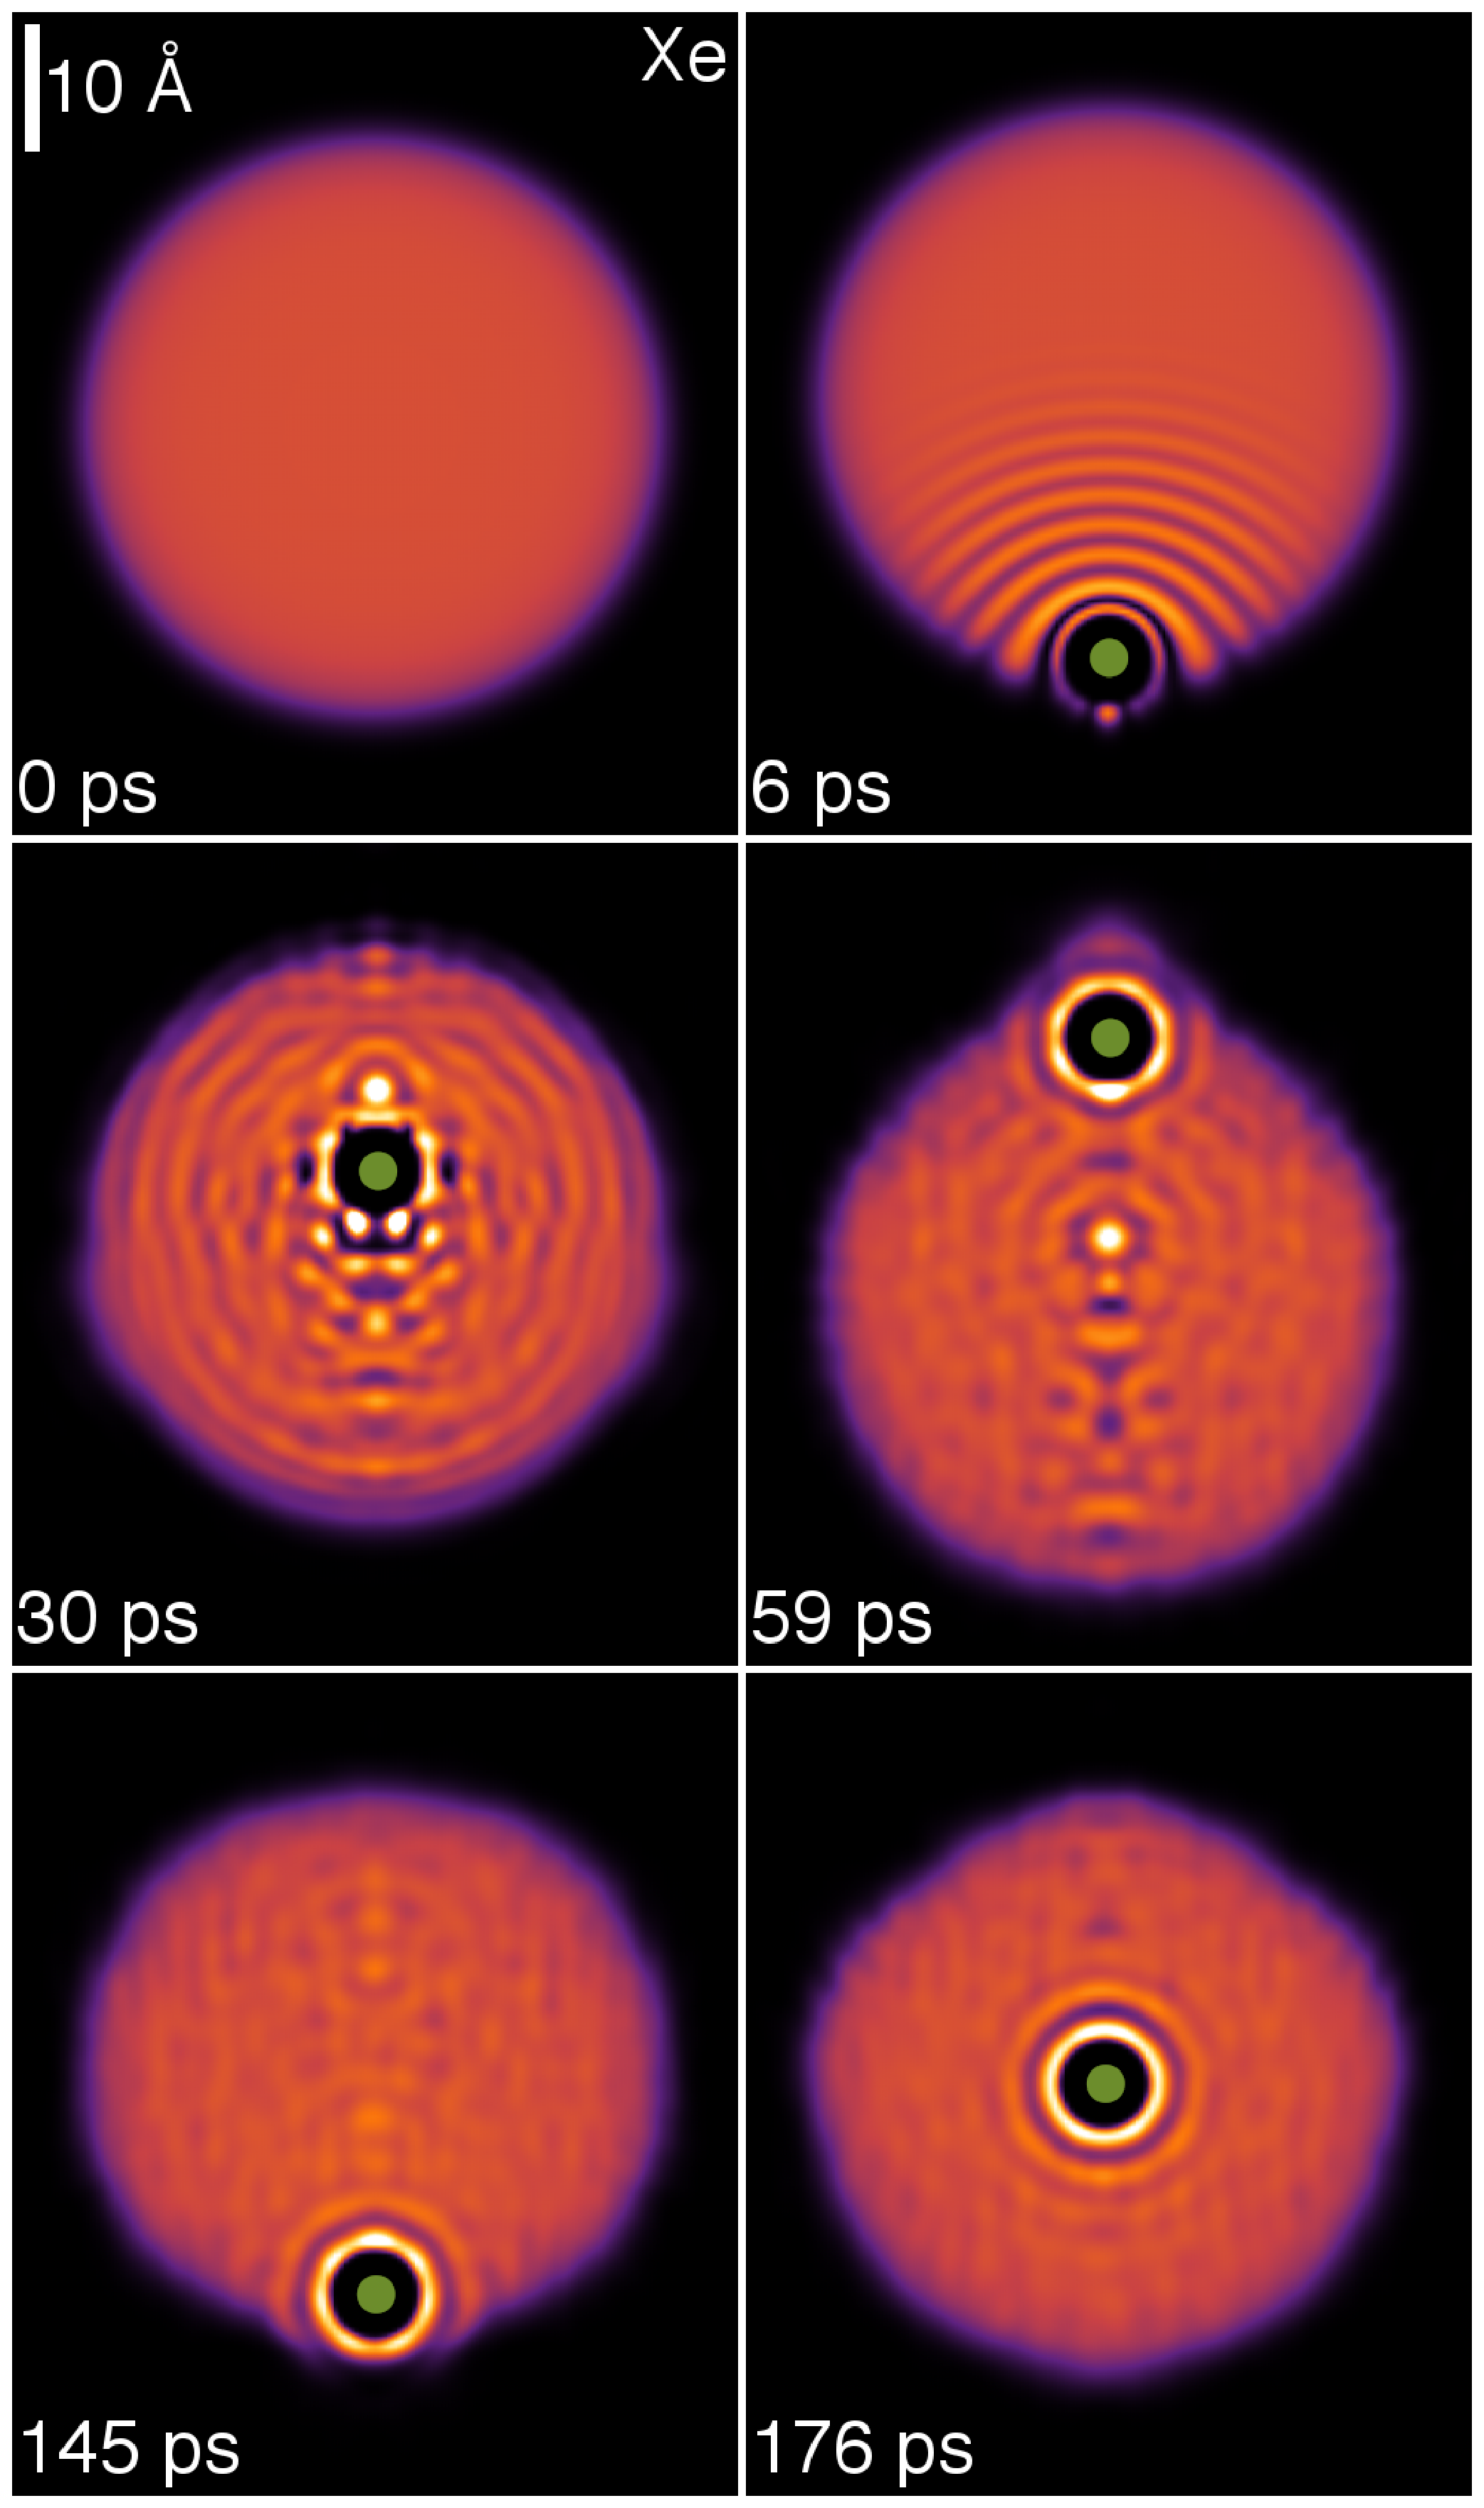
\includegraphics[width=0.50\linewidth,clip]{fig2-Xe}}
			\caption{\label{fig2-headon}Right panel: Dynamic evolution of a Xe atom (big dot) approaching the $^4$He$_{1000}$ droplet from below at $v_0 = 200$ m/s. The corresponding time is indicated in each frame. Left panel: Same as left figure for a Cs atom. (Color figure online.)}
		\end{figure}

		\begin{figure}[!]
			\centerline{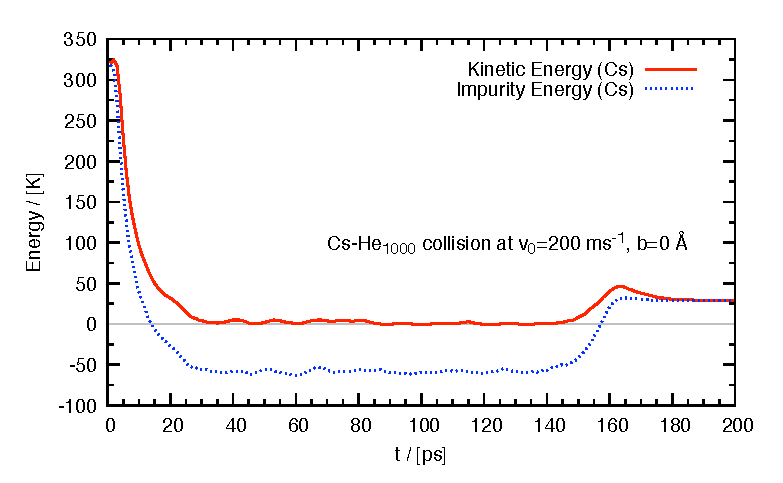
\includegraphics[width=0.90\linewidth,clip]{fig3-Cs-He}} 
			\centerline{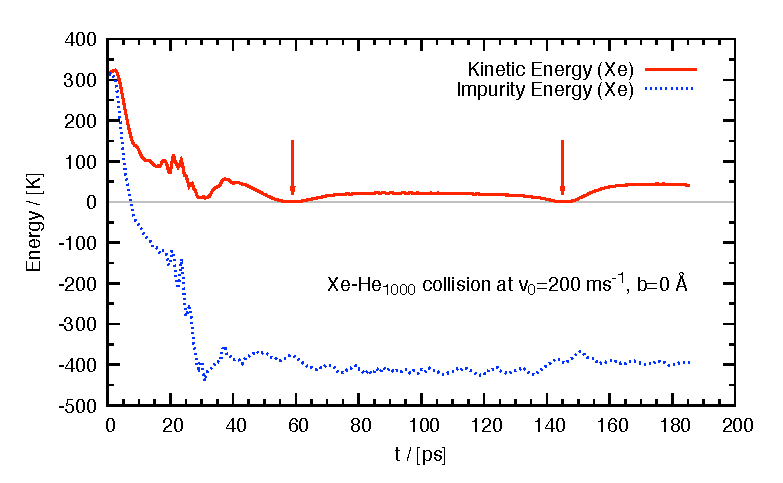
\includegraphics[width=0.90\linewidth,clip]{fig3-Xe-He}}
			\caption{\label{fig3-headon}Top figure: Kinetic and total (kinetic plus potential) energy as a function of time  of a Cs atom head-on colliding against a  $^4$He$_{1000}$ droplet at  $v_0 = 200$ m/s. Bottom figure: same as top figure for a Xe atom. The vertical arrows indicate the first two turning points at 59 and 145 ps, whose corresponding helium densities are shown in the right \fig{fig2-headon}. (Color figure online.)}
		\end{figure}

		We consider a droplet made of $N=1000$ helium atoms. Its ground state structure is obtained using DFT and gives a sharp-density  radius of about 22.2 \AA{}. Then the dynamics is initiated by placing the Xe atom 32 \AA{} away from the center of mass (COM) of the droplet with an impact parameter equal to zero (head-on collision). The simulations are carried out for initial Xe velocities  $v_0$ ranging from 200 to  600 m/s in the system of reference of the droplet, corresponding to kinetic energies between  315.8 K and  2842 K. These energies can be compared to the solvation energy of a Xe atom at the center of a $^4$He$_{1000}$ droplet, $S_{{\rm Xe}} = E({\rm Xe}@^4{\rm He}_{1000}) - E(^4{\rm He}_{1000}) = -316.3$ K. For the sake of comparison, the solvation energy of Cs is -5.2 K and its equilibrium position is  in a dimple at the outer droplet surface, about 26.6 \AA{} from its centre. 

		Thermal Xe atoms ($v_0 \sim$ 240 m/s) are used in the experiments\citep{Gom14,Jon16}, and the average droplet velocity is about 170 m/s\citep{Gom11}.

		\fig{fig1-headon} shows the energy of  the Xe@$^4$He$_{1000}$ complex  referred to that of the equilibrium configuration (Xe at the center of the droplet, $-5716.4$ K) as a function of the distance between the Xe  atom and  the COM of the droplet. It is obtained by a constrained calculation similar to that presented in\rf{Lea16} for Ba$^+$. 
With increasing distance, the stretched droplet-Xe configuration eventually breaks into a minicluster around the Xe atom containing 
about 22 helium atoms disconnected from the rest of the droplet.
The appearance of this minicluster is at variance with the situation for a heliophobic impurity such as Cs\citep{Lea14a}.
The stretched (connected) configuration energies are represented by dots, the disconnected ones by triangles.
The two corresponding curves cross at  37 \AA{}.
At shorter distances the connected configuration is stable and the disconnected one metastable, and at larger distances the roles are inverted.
In an actual dynamics the number of He atoms in the minicluster  depends on the velocity of the Xe projectile.

 \fig{fig2-headon} displays two-dimensional plots of the helium density for Xe  head-on  colliding against the $^4$He$_{1000}$
 droplet at $v_0=$ 200 m/s, and \fig{fig3-headon} the energy of the impinging atom as a function of time,
 with the corresponding plots for Cs collisions for the sake of comparison.  It can be seen that for both species
 most of the initial kinetic energy is spent in piercing the droplet surface, after which the impurity moves inside the droplet  
at a velocity  well below the critical Landau velocity  $v_L$. 
 
\fig{fig2-headon} also shows that the collision launches a series of density waves in the droplet 
  that are reflected at the droplet free surface producing  complex interference patterns in
 its bulk. As an illustrative example, \fig{fig4-headon} shows the density profile along the incident direction ($z$ axis) corresponding to the Xe collision at $v_0=$
 200 m/s, 6 ps after the process starts.
 The wave number  associated to this  wave can be estimated from the wavelength $\lambda$  of the 
  oscillations, $q = 2 \pi/\lambda \sim$ 2.7 \AA$^{-1}$.

\begin{figure}[!]
\centerline{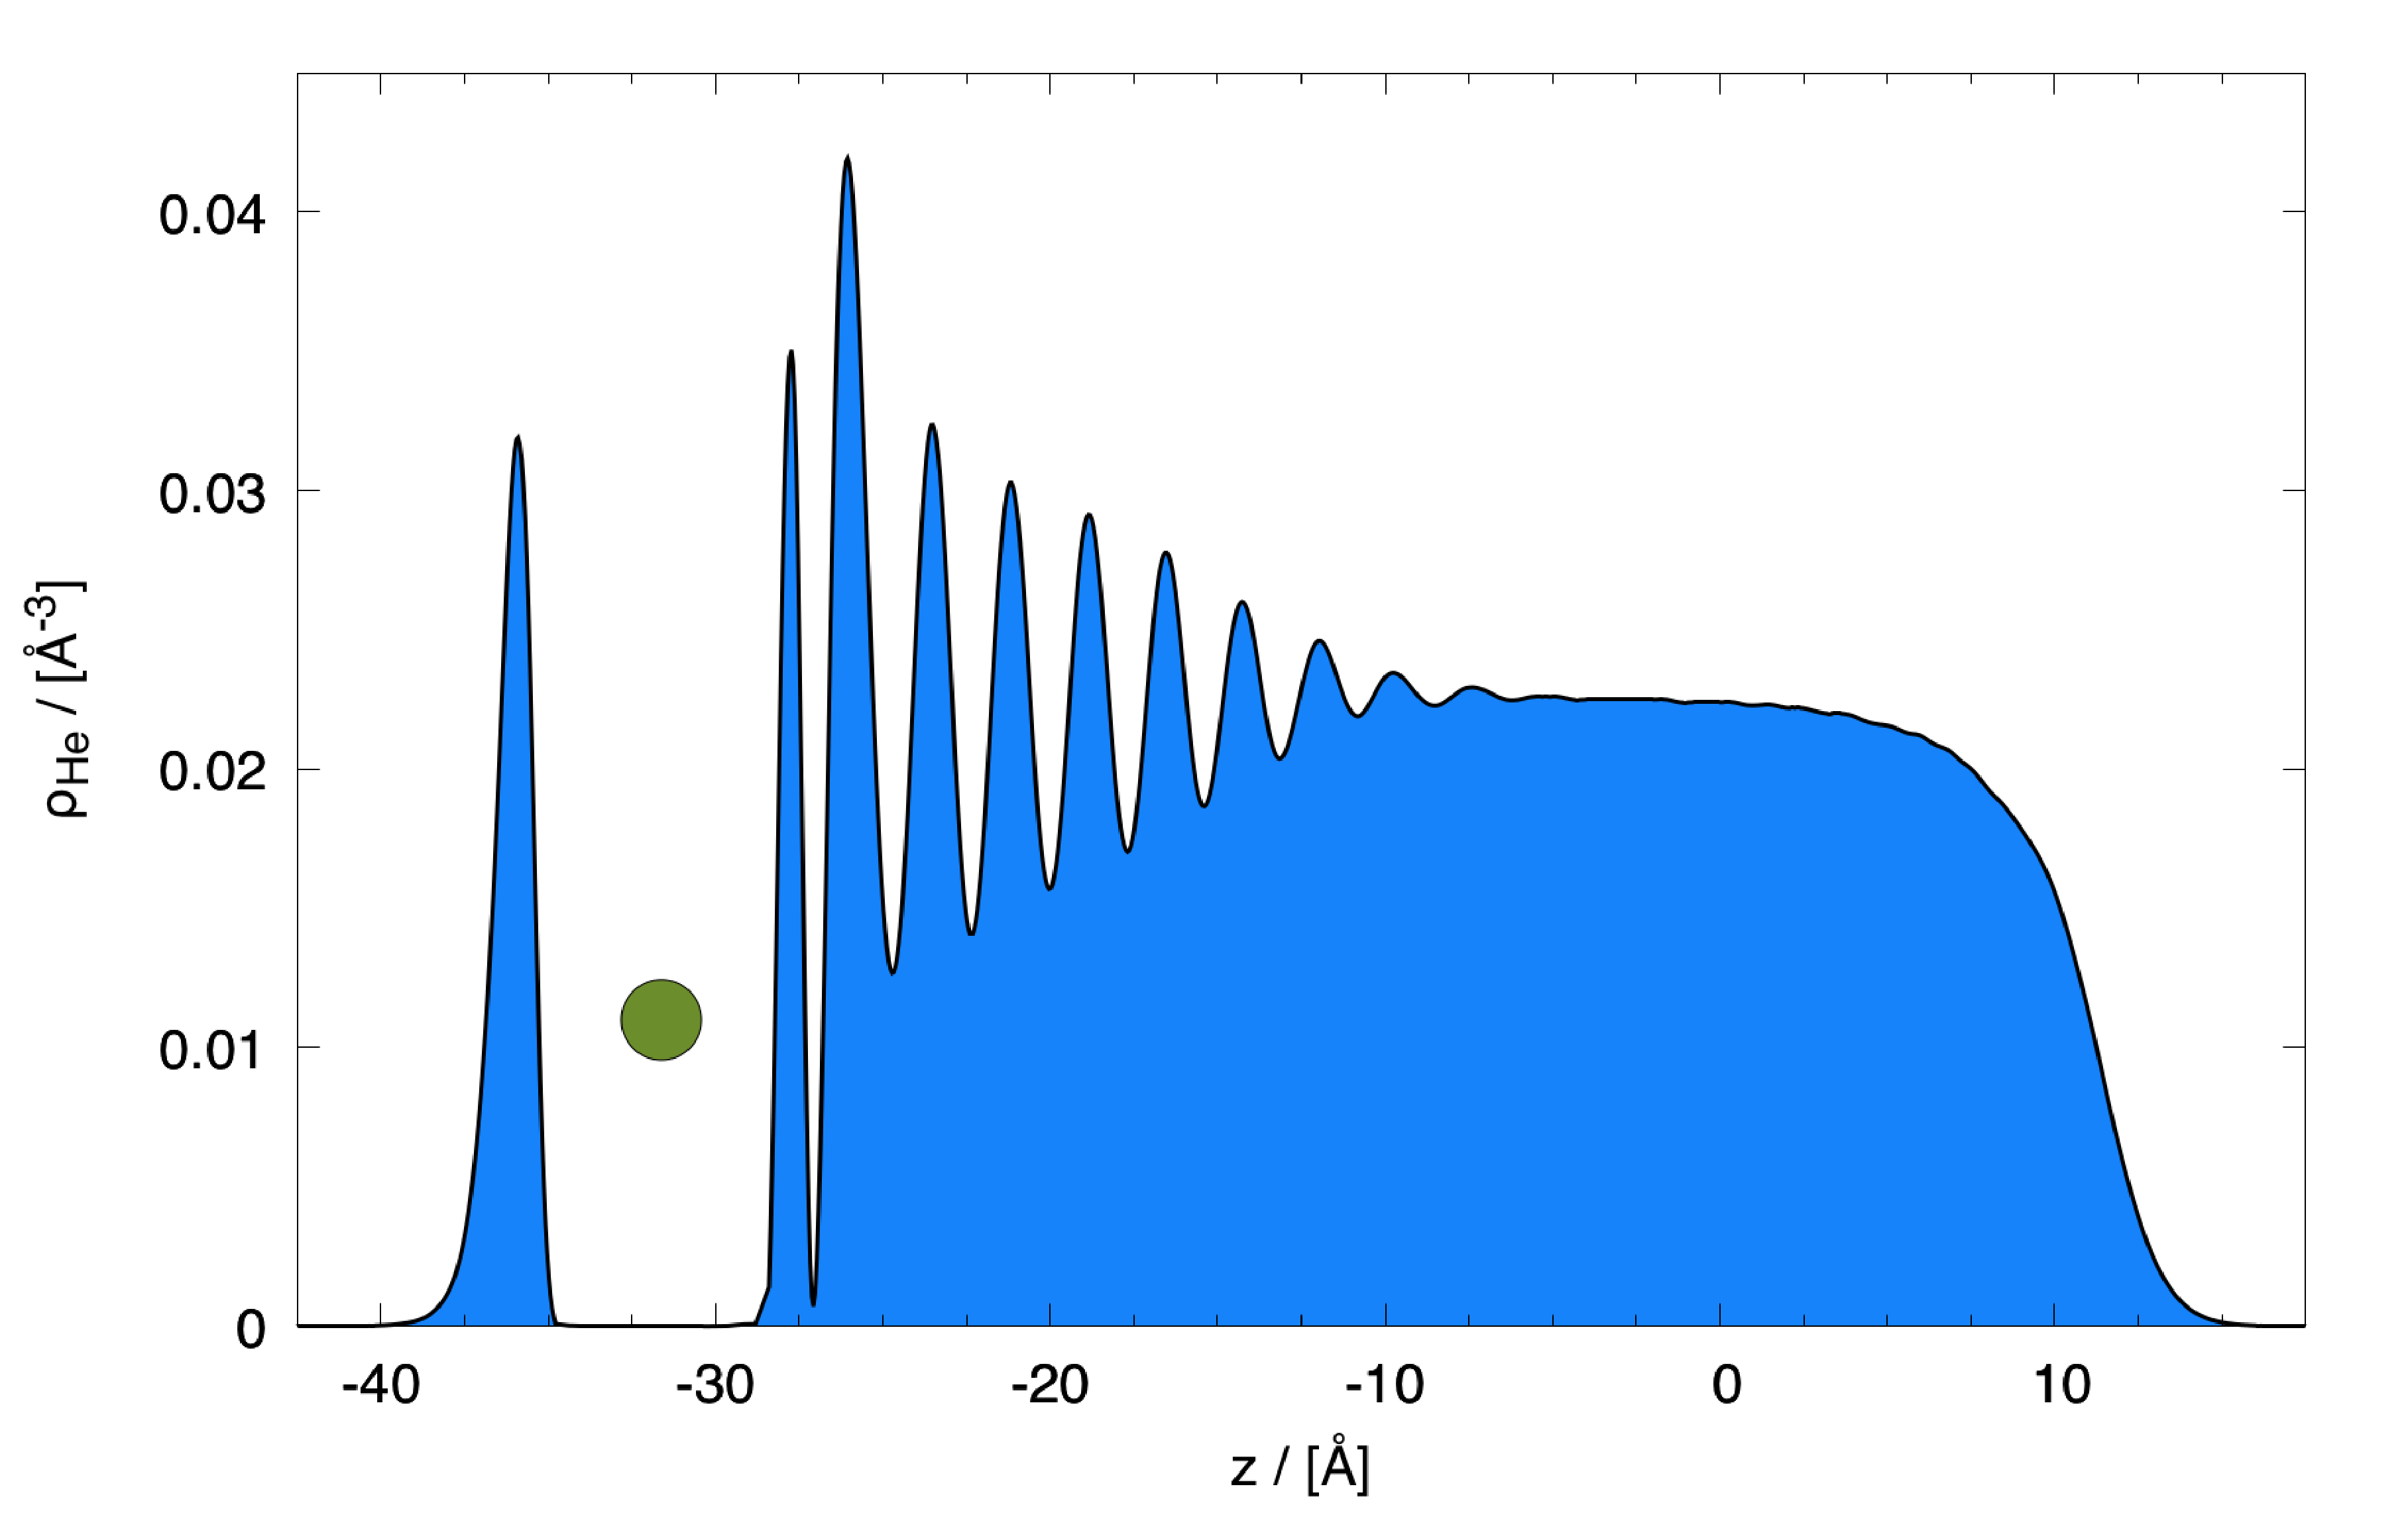
\includegraphics[width=0.90\linewidth,clip]{fig4}} 
\caption{\label{fig4-headon} 
Density profile of the He$_{1000}$ droplet along the incident direction corresponding to the Xe collision at $v_0=$
 200 m/s after 6 ps. (Color figure online.)
}
\end{figure}

In the case of Xe, \fig{fig2-headon} and \fig{fig3-headon}  reveal the appearance of turning points at which the velocity of the impurity is zero.
Note that these points are not fixed during the dynamics since the droplet deforms due to the swift motion of Xe inside it; 
the droplet is not a rigid object and reacts to the motion of the impurity, with  energy being transferred not only from the impurity 
to the droplet but also the other way around\citep{Mat14}.

The top left inset in \fig{fig1-headon} shows a snapshot obtained at the first turning point for $v_0=$ 600 m/s, with 57 He atoms around the Xe dopant.
We have found that the Xe atom has to hit the droplet at a velocity above 600 m/s  in order to go across the helium droplet, otherwise it remains attached to the droplet.
The kinetic energy lost by the Xe atom is partially deposited in the droplet and partially carried away by prompt-emitted helium atoms, \textit{i.e.} atoms expelled 
early on in the collision and with a significant kinetic energy. The number of He atoms 
 emitted during the first 78 ps is about 47. For comparison, about 19 atoms are emitted after 185 ps for $v_0$ = 200 m/s. 
 Eventually, the energy deposited into the droplet should be lost by atom evaporation; however, the time scale for this to happen is 
 beyond the reach of any realistic simulation. 
 
 
\begin{figure}[!]
\centerline{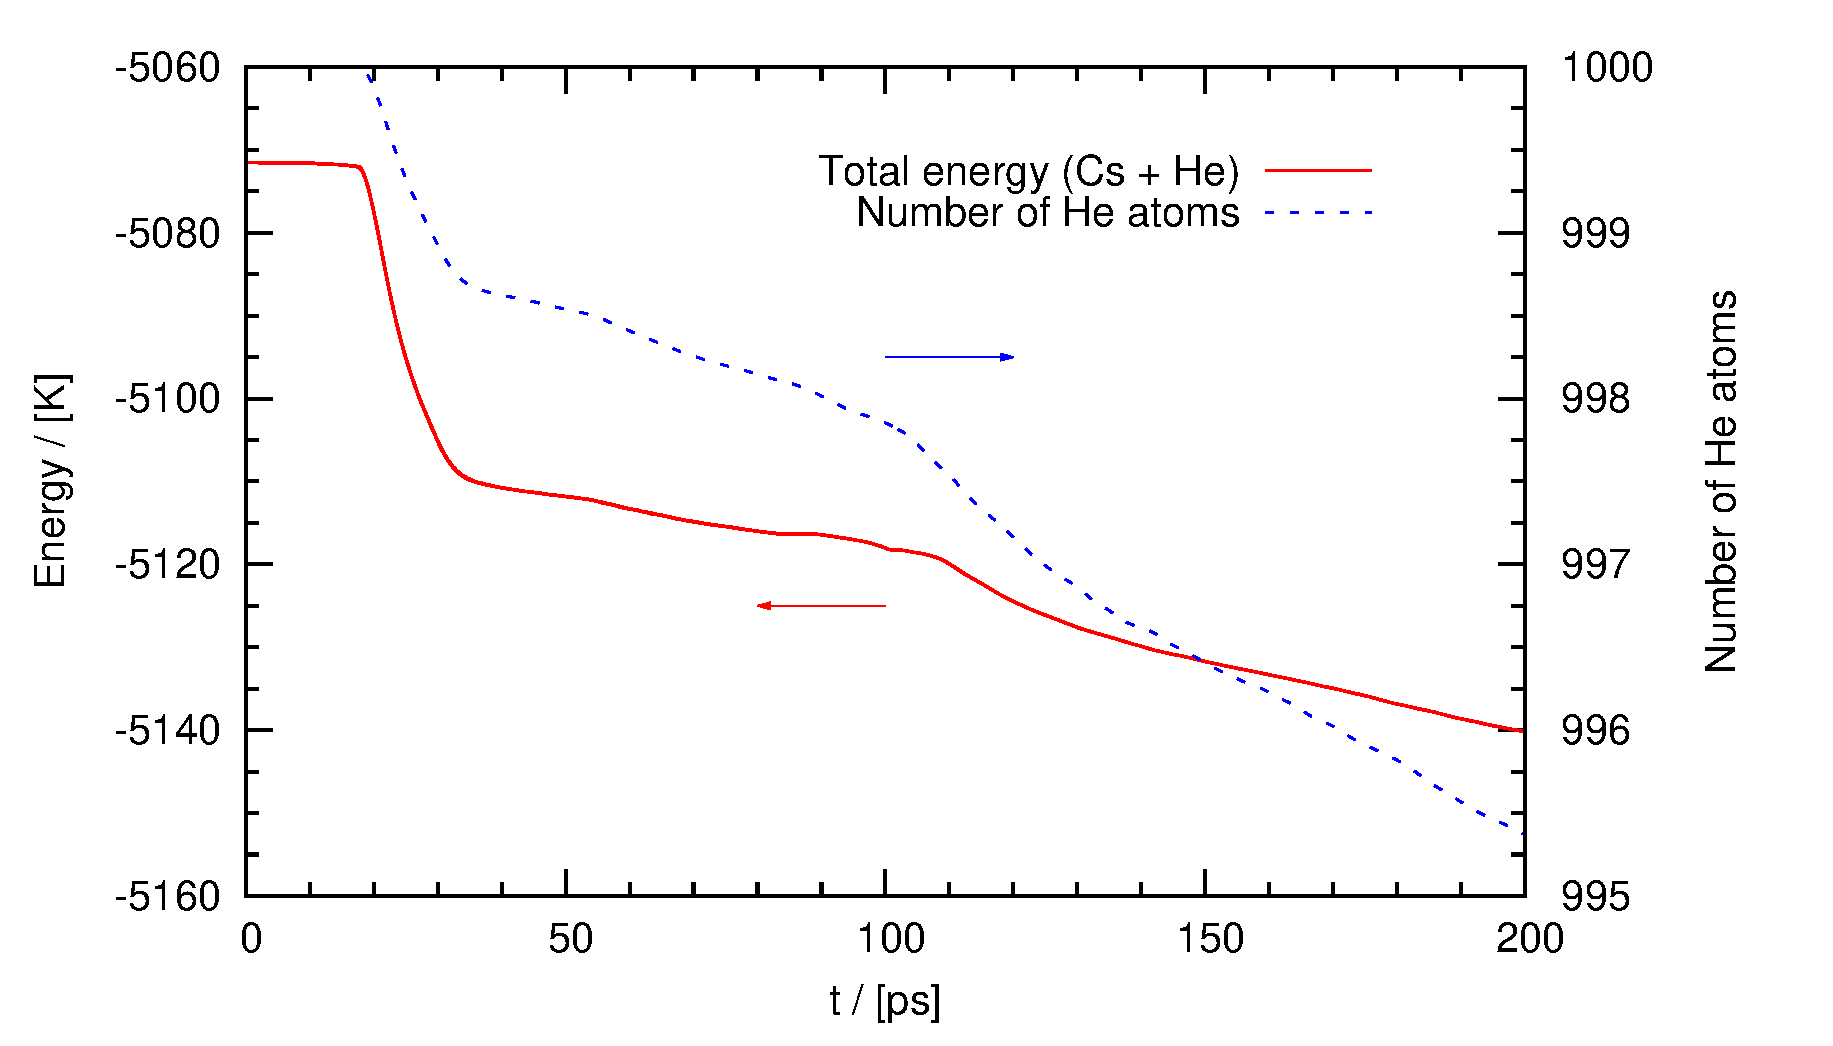
\includegraphics[width=0.90\linewidth,clip]{fig5}}
\caption{\label{fig5-headon} 
Total energy  (left scale) and number of atoms in the droplet (right scale) as a function of time for the 
Cs@$^4$He$_{1000}$ system at $v_0 = 200$ m/s. (Color figure online.)
}
\end{figure}

 
 The piercing of the droplet by the Cs atom produces a density wave that travels on its surface and collapses at the surface region opposite to the hitting point.
 This collapse nucleates a 
 vortex ring (the two dark spots in the 76 ps plot of the left panel of \fig{fig2-headon})\citep{Lea14a}.
 
 It is worth pointing out that the falloff of the Xe velocity in the $t=20-30$ ps interval observed in \fig{fig3-headon}  is due to the increase of its inertia
due to the appearance of a dynamic ``snowball''  --a crust of helium atoms surrounding the Xe bubble indicated by the bright spots in 
\fig{fig2-headon}-- that is eventually washed out at larger times.
At variance with our findings for Ba$^+$\citep{Mat14}, vortex rings have not been nucleated in the case of Xe; in particular, we have checked that the two dark spots  in the 30 ps plot of the right panel of \fig{fig2-headon} for Xe do not correspond to a vortex ring. 

The collapse of the Cs bubble at the surface of the droplet some 150 ps after the process 
 gives back to the impurity part of the kinetic energy it has lost  in the 
 piercing of the droplet. The Cs atom is expelled at 64.5 m/s (corresponding to 33.6 K kinetic energy). 
The number of prompt-emitted helium atoms is 5, which is smaller than for Xe at the same collision energy (19 atoms).
As revealed by \fig{fig5-headon}, they are  preferentially emitted as a forward  burst  (first sharp drop around 20 ps in the number of atoms) and as a 
backward burst  (second sharp drop slightly after 100 ps).
